\appendices
\section{Classifier Architecture and Calibration}
\label{app:ablation}
\begin{figure*}[t]
\centering
% Panel crops of the old ablation.png (Figures/exp_frames/ab_*.png);
% regenerate from matplotlib (same filenames) for print quality.
\resizebox{\textwidth}{!}{%
\begin{tikzpicture}[font=\small,
  photo/.style={inner sep=0pt, draw=gray!40, thin},
  lbl/.style={font=\scriptsize, align=center}]
\node[photo] (a) {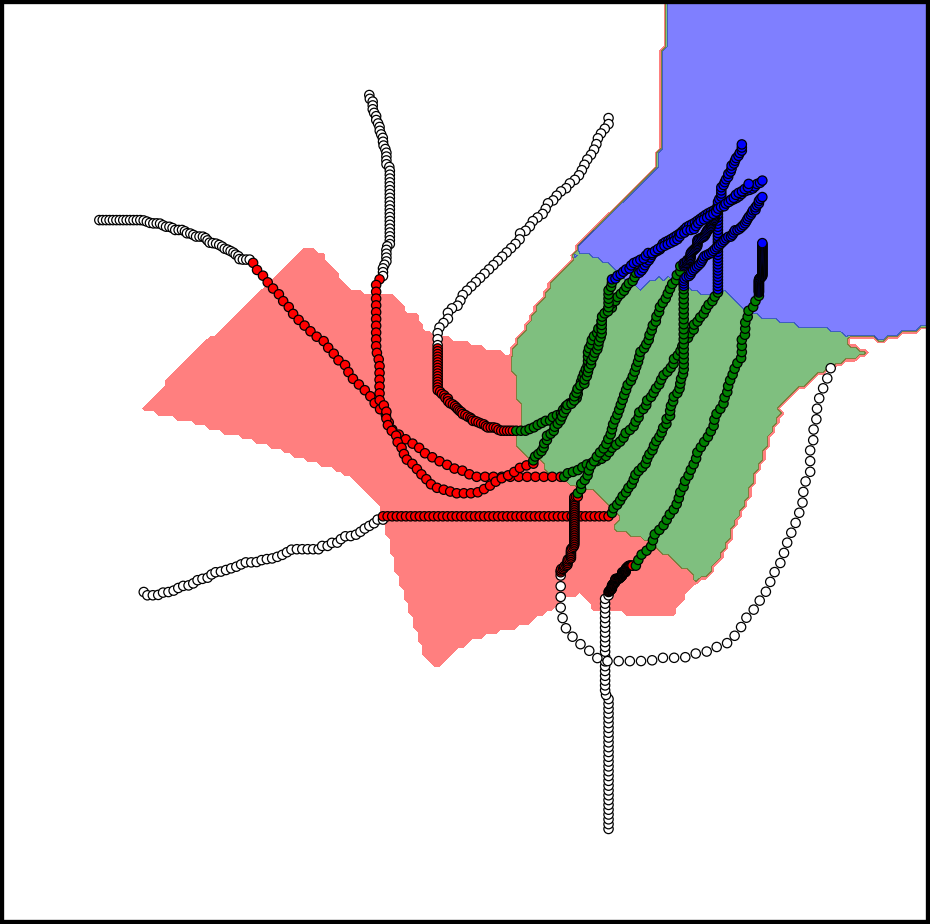
\includegraphics[width=3.2cm]{Figures/exp_frames/ab_knn.png}};
\node[photo, right=2mm of a] (b) {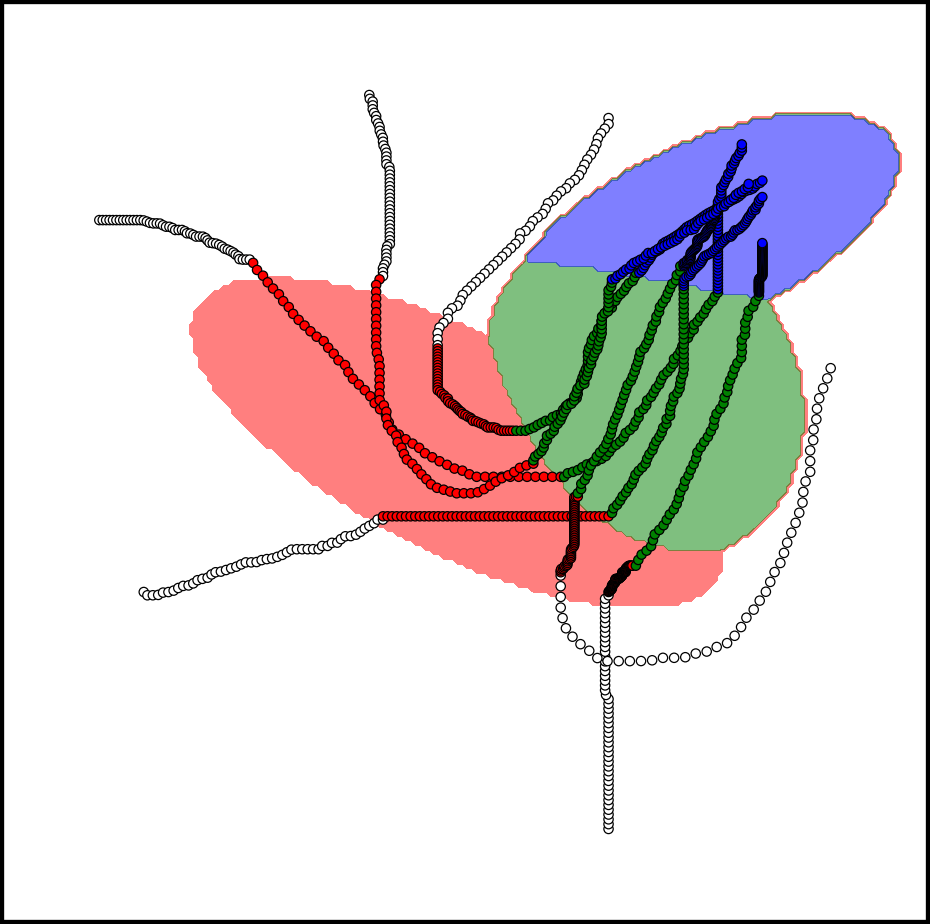
\includegraphics[width=3.2cm]{Figures/exp_frames/ab_lr.png}};
\node[photo, right=2mm of b] (c) {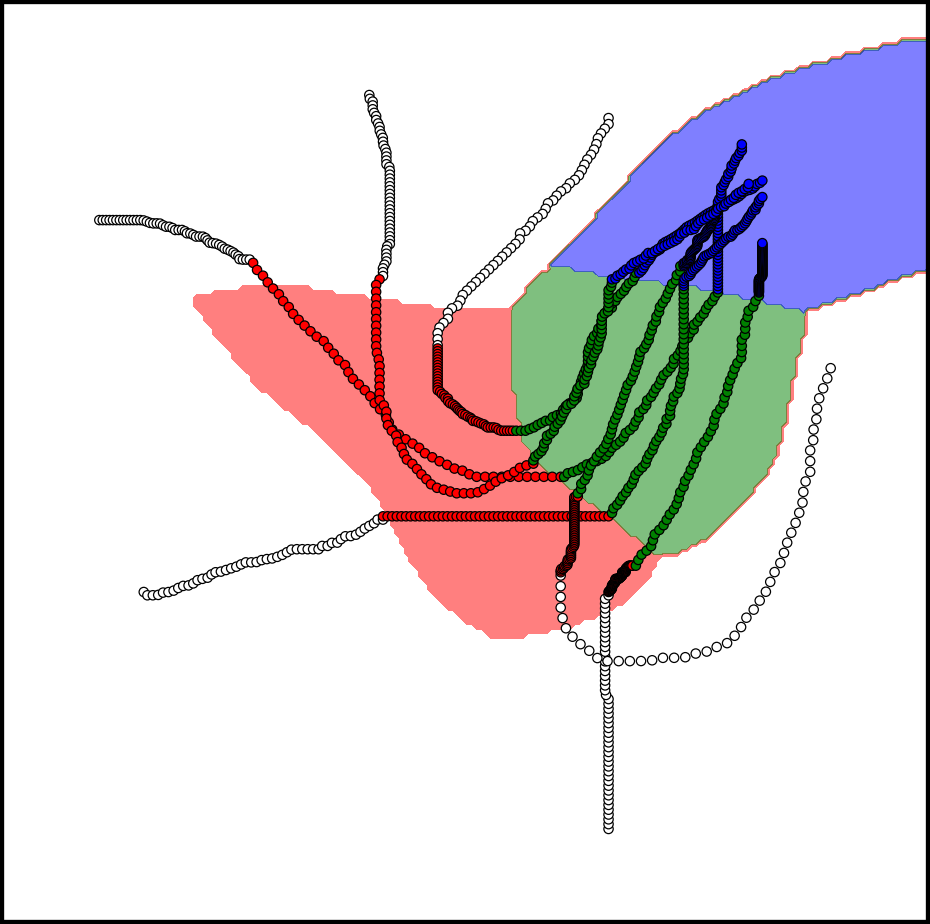
\includegraphics[width=3.2cm]{Figures/exp_frames/ab_mlp.png}};
\node[photo, right=2mm of c] (d) {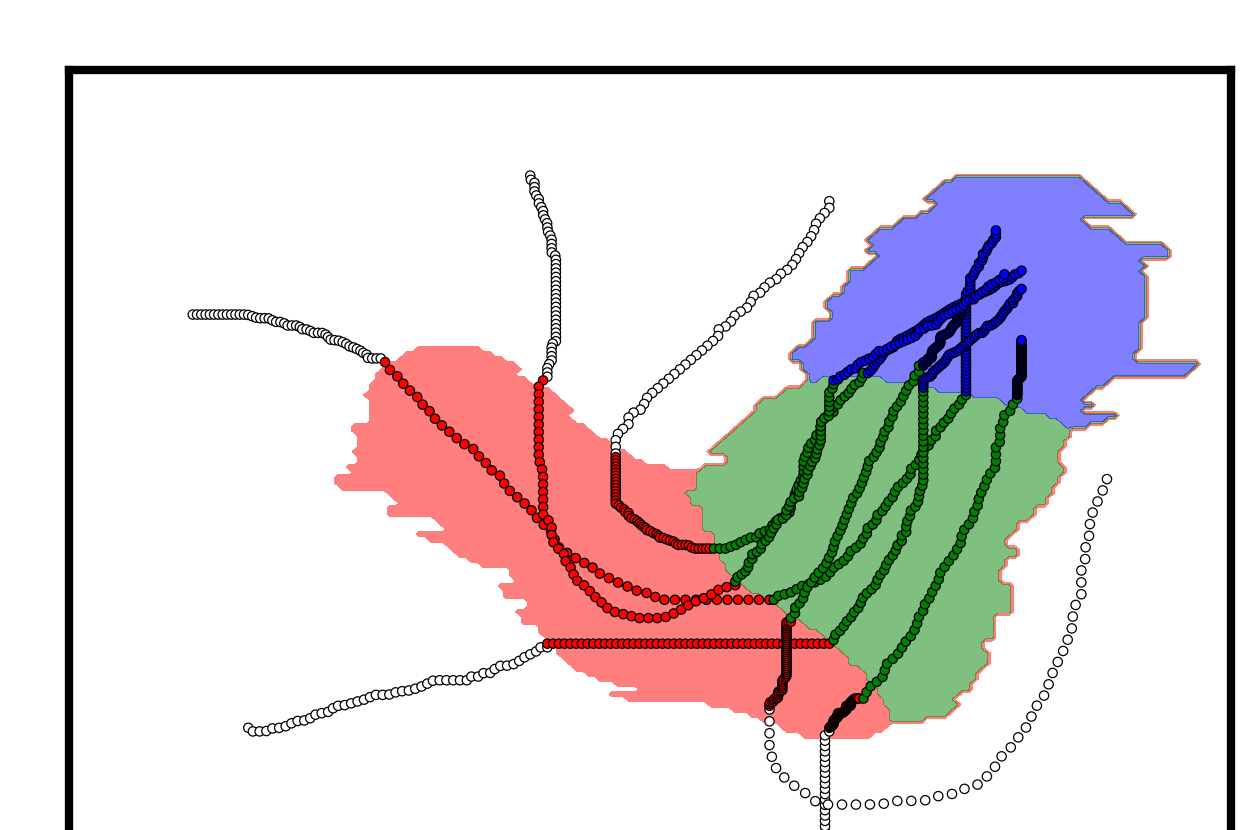
\includegraphics[width=3.2cm]{Figures/exp_frames/ab_seal.png}};
\node[photo, right=2mm of d] (e) {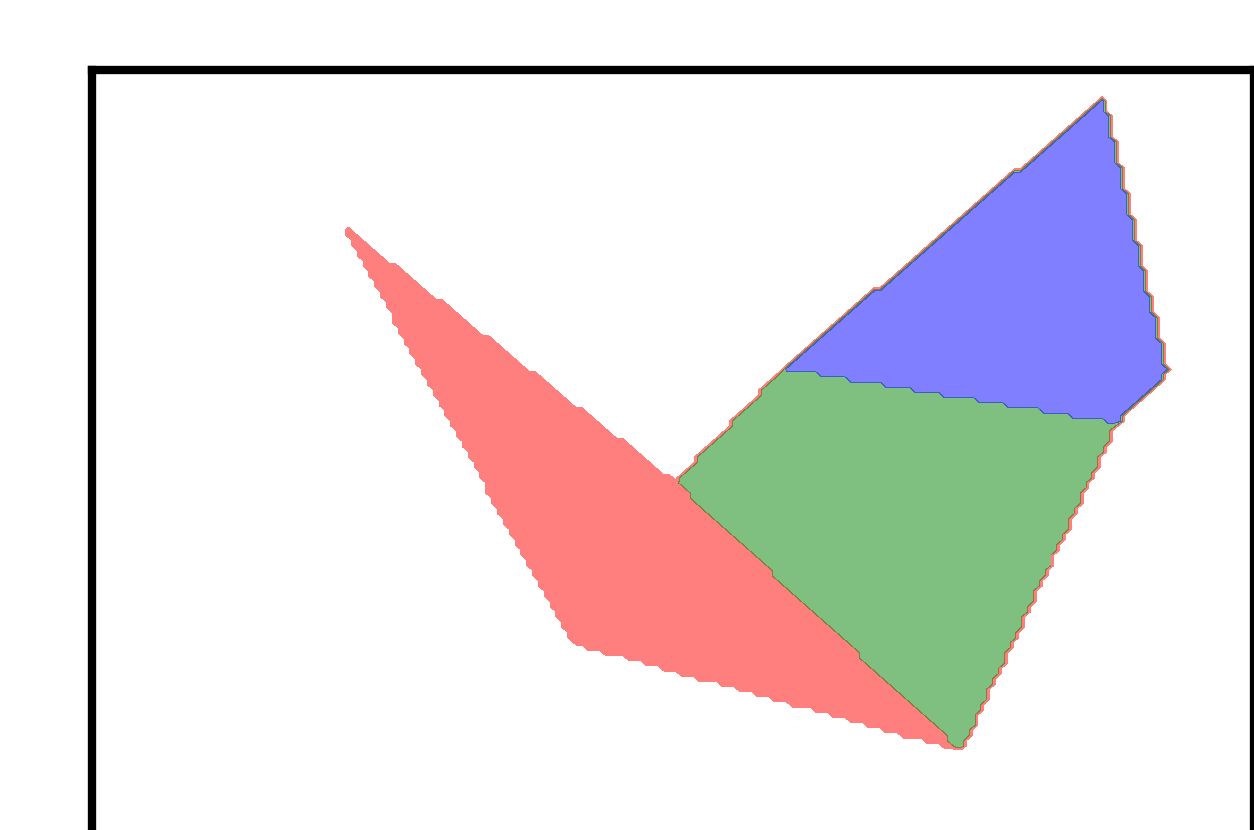
\includegraphics[width=3.2cm]{Figures/exp_frames/ab_gt.png}};
\node[lbl, above=0.5mm of a] {(a) $k$-NN, mIoU 0.670};
\node[lbl, above=0.5mm of b] {(b) logistic regr., mIoU 0.721};
\node[lbl, above=0.5mm of c] {(c) MLP, mIoU 0.725};
\node[lbl, above=0.5mm of d] {(d) \textbf{SEAL (GPC), mIoU 0.820}};
\node[lbl, above=0.5mm of e] {(e) ground truth};
\node[photo, below=6mm of a] (f) {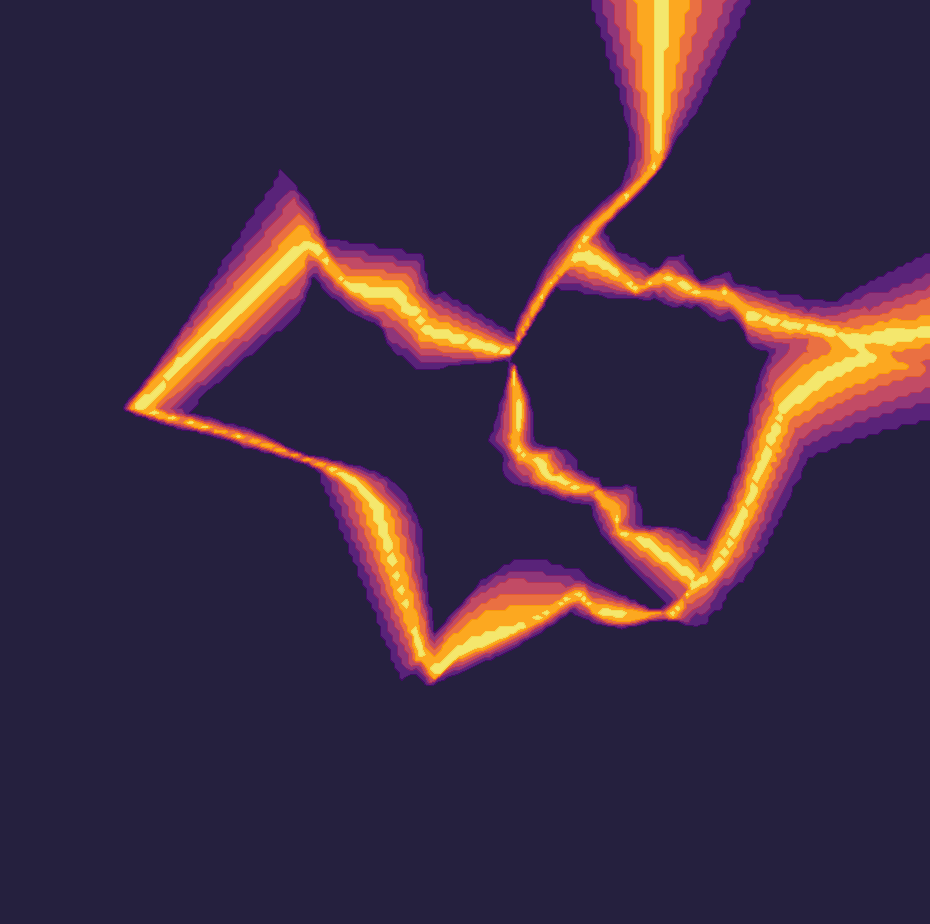
\includegraphics[width=3.2cm]{Figures/exp_frames/ab_knn_u.png}};
\node[photo, right=2mm of f] (g) {
\includegraphics[width=3.2cm]{Figures/exp_frames/ab_lr_u.png}};
\node[photo, right=2mm of g] (h) {
\includegraphics[width=3.2cm]{Figures/exp_frames/ab_mlp_u.png}};
\node[photo, right=2mm of h] (i) {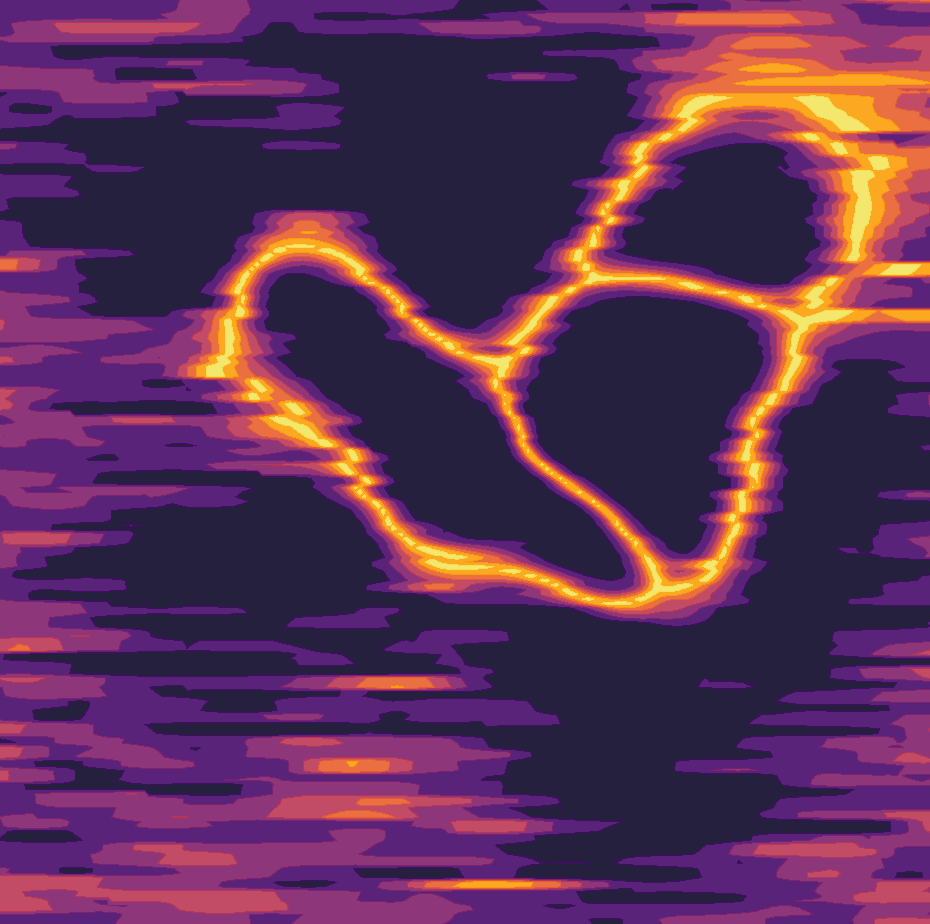
\includegraphics[width=3.2cm]{Figures/exp_frames/ab_seal_u.png}};
\node[photo, right=2mm of i] (j) {
\includegraphics[width=3.2cm]{Figures/exp_frames/ab_seal_epi.png}};
\node[lbl, below=0.5mm of f] {(f) $k$-NN margin unc.};
\node[lbl, below=0.5mm of g] {(g) logistic margin unc.};
\node[lbl, below=0.5mm of h] {(h) MLP margin unc.};
\node[lbl, below=0.5mm of i] {(i) SEAL margin unc.};
\node[lbl, below=0.5mm of j] {(j) SEAL epistemic unc.};
\end{tikzpicture}%
}
\caption{\textbf{Classifier ablation on 2D navigation.} Top row: learned mode regions and mIoU per model against the ground truth (e). Bottom row: uncertainty landscapes; only the GPC exposes an epistemic component (j) that grows in the unobserved top-right region, while the MLP (h) remains confident there.}
\label{fig:ablation}
\end{figure*}
\textbf{Implementation details.} \todo{state the GPC implementation: number of inducing points $M$, kernel and initialization, variational distribution, optimizer and iterations, and training time per round} \todo{LATENCY BENCHMARK (co-author): the paper claims monitoring ``at upwards of 30\,Hz'' (Sec.~II), i.e., single-observation prediction must take $<$33\,ms. On the machine actually used for robot deployment, time $f(\mathbf{x})$ (posterior mean + variance, batch size 1, including feature extraction if nontrivial) averaged over $\geq$1000 calls, for the trained models of each task, and sweep dataset size and $M$ (e.g., $M\in\{32,64,128,256\}$) to show the scaling. Report a small table or plot (ms vs.\ $M$/dataset size) + the achieved Hz per task. If any deployed configuration misses 33\,ms, soften the 30\,Hz claim in Sec.~II rather than defend it.}

\textbf{Classifier ablation.} We ablate the classifier on the simulated 2D Navigation task, replacing the GPC with an MLP, logistic regression, and $k$-NN, all trained on the same data (\todo{state the hyperparameter-tuning protocol used for the baselines, so the comparison is demonstrably fair}) (Fig.~\ref{fig:ablation}). The simpler $k$-NN and logistic models underfit; the MLP comes closest among the baselines to the GPC's mIoU. However, unlike an MLP, which is overconfident far from training data, the GPC's posterior uncertainty grows where samples are sparse (Fig.~\ref{fig:ablation}f--j): the top-right region, unobserved in the initial demonstrations, is correctly flagged as uncertain by the GPC (i) while the MLP (h) stays confident. The GPC yields epistemic uncertainty (j) directly, without the expensive ensembling or MC-dropout other models require, and this drives active queries into informative, unexplored regions, making learning robust to sub-optimal initial demonstrations. \textbf{Calibration.} Because our confidence gating relies on the variational posterior, which can under-estimate uncertainty, we report a reliability diagram of the gated confidences and the resulting choice of $\tau$: \todo{CALIBRATION (co-author): on held-out labeled data (e.g., leave-one-demo-out per task, or the 2D-nav ground truth), bin the GPC's predicted confidence $prob^*$ into 10 bins and plot empirical accuracy per bin vs.\ confidence (reliability diagram); report ECE as the summary number. State the $\tau$ actually used in the experiments and mark it on the diagram; the claim to support is that at $prob^*>\tau$ the empirical accuracy is high enough to justify gating. If the variational posterior is overconfident (curve below diagonal), say so and note $\tau$ was chosen conservatively---do not hide it.}. \textbf{Product kernel vs.\ independent GPs.} On the Stack task we compare the product kernel against fitting an independent GP per gripper state: \todo{PRODUCT-KERNEL ABLATION (co-author): on the Stack task, train (a) the product-kernel GPC and (b) one independent GPC per gripper context, on identical data, and report mIoU (or task success over the same 100 episodes) for both---expected: parity with 2 contexts. For the scaling claim, either add a task/variant with $>$2 discrete contexts (e.g., gripper state $\times$ object type) showing the independent-GP ensemble degrades as per-context data thins while the shared-$\mathbf{B}$ product kernel does not, or SOFTEN the sentence in Sec.~IV-C to a data-splitting argument without the empirical claim.}.

\section{Feature Selection: A Worked Example}
\label{app:feature}
The prompt supplied to the LLM in Stage~1 (Fig.~\ref{fig:framework}a) consists of a task-specific part and a fixed template:
\begin{itemize}
\item \textbf{Task-specific:} the task description (e.g., ``this is a pick and place task\,\dots''), the available raw features ($F_{\text{raw}}$, e.g., \texttt{EE\_pos}, \texttt{EE\_orn}, \texttt{Bottle\_pos}, \dots), and the target modes (e.g., \textit{Pick}, \textit{Transport}, \textit{Place}).
\item \textbf{Fixed template:} the LLM is instructed to act as a robotics engineer, to think \emph{prescriptively rather than descriptively}, to account for failures and perturbations, and to return a minimal list of processed features favoring spatially invariant relative quantities over absolute coordinates.
\end{itemize}
We argue that MI alone is insufficient for feature reduction: in the few-shot regime it cannot separate causal geometry from spurious spatial correlation. For instance, in restocking, replacing the relative end-effector-to-bottle angle with the \emph{absolute} angle yielded nearly identical MI, so MI cannot filter spatially dependent features; hence the LLM's invariance prior is required before mathematical verification. The following illustrates the end-to-end pipeline, showing how the MI certificate rejects an under-specified prompt and how ablation prunes the corrected set.

\textbf{Phase 1 (initial, under-specified prompt).} The operator omits that the bottle starts inside the basket:
\begin{quote}\small\itshape ``The objective is to restock the bottle onto the shelf. The robot must first establish a top grasp to lift the carton, place it on the table, transition to a side grasp, and finally place it on the shelf.''\end{quote}
The LLM proposes \{\textit{is\_grasped}, \textit{relative\_alignment}, \textit{z\_dist\_table}, \textit{z\_dist\_shelf}\}, whose $X_{\text{sel}}$ yields a joint MI of only $1.1036$ nats, well below the raw baseline $I(X_{\text{raw}};Y)\approx1.2737$ nats. The verification layer rejects it and requests a more descriptive prompt. (The raw baseline sits below the theoretical maximum $H(Y)=\ln 4\approx1.386$ nats because points near guards are intrinsically ambiguous and the $k$-NN estimator is biased at small sample sizes; the sufficiency test therefore compares against the empirical raw baseline, not against $H(Y)$.) \todo{verify: the Phase-1 MI ($1.1036$) is identical to four decimals to the ``Drop $d_{\text{basket}}$'' entry in the Phase-3 table, although the two feature sets differ---check both values against the experiment logs}

\textbf{Phase 2 (corrected prompt).} The operator adds the physical bottleneck:
\begin{quote}\small\itshape ``\dots When the carton is inside the basket, the robot can only grasp it from the top. If the carton is grasped from the top, the robot must place it on the table and regrasp it from the side before placing it on the tight shelf.''\end{quote}
The LLM outputs a spatially invariant set: $d_{\text{basket}}$ (carton--basket distance), $is_{\text{held}}$ (gripper boolean), $\theta_{\text{rel}}$ (end-effector--carton angle), and $h_{\text{carton}}$ (absolute carton height). Notably $h_{\text{carton}}$ is an absolute coordinate that slips through the invariance prior, an intentional illustration that the LLM can still propose a suboptimal feature, which the following minimization catches. This set yields $1.2704$ nats, matching the baseline; the system accepts it and proceeds.

\textbf{Phase 3 (minimization).} Dropping each feature and recomputing MI:
\begin{center}
\resizebox{\columnwidth}{!}{%
\begin{tabular}{@{}llc@{}}
\toprule
\textbf{Feature Set} & \textbf{MI (nats)} & \textbf{Information Loss ($\Delta$)} \\ \midrule
Full 4D Set (Baseline) & 1.2704 & -- \\ \midrule
Drop $d_{\text{basket}}$   & 1.1036 & $-0.1668$ (Critical) \\
Drop $is_{\text{held}}$    & 1.1429 & $-0.1275$ (Critical) \\
Drop $\theta_{\text{rel}}$ & 1.2399 & $-0.0305$ (Critical) \\
Drop $h_{\text{carton}}$   & \textbf{1.2706} & $\mathbf{+0.0002}$ (Redundant) \\ \bottomrule
\end{tabular}%
}
\end{center}
A drop is marked \emph{Critical} when the loss exceeds the same tolerance $\epsilon$ used in the sufficiency check (Sec.~\ref{sec:feature_engineering}), and \emph{Redundant} otherwise; the $+0.0002$ nat ``gain'' from dropping $h_{\text{carton}}$ is within estimator noise. Omitting the absolute coordinate thus incurs zero information loss, and it is discarded, finalizing the causally robust 3D space $F_{\min}=[d_{\text{basket}},is_{\text{held}},\theta_{\text{rel}}]$.
